\documentclass[12pt,oneside,reqno]{article}
\usepackage[utf8]{inputenc}
\usepackage[left=3cm,right=3cm,top=2.5cm,bottom=2.5cm]{geometry}
\usepackage{amsmath,amsfonts,amssymb,xfrac,xcolor,placeins,subcaption}
\usepackage{enumitem}
\usepackage{fancyhdr}
\pagestyle{fancy}

\newcommand{\pr}{\mathbb{P}\mathrm{r}}

\title{Assignment II}
\author{Jose M. Quintero\thanks{https://github.com/jmquintero925/Int.-Macro-and-Trade}}
% \date{October 2022}
%\thanks{I collaborated with Lauren Mostrom}

\lhead{Jose M. Quintero}
\rhead{Int. Macro and Trade.} 

\begin{document}

\maketitle 
\section{Quantitative Model}

We start with the simplest version of the EK model seen in class augmented to have trade imbalances. Specifically, consider the same environment of EK (2002) introduced in week 2 that features multiple countries, a single sector, and production functions that use only labor. We then extend the model to allow for trade imbalances: total spending in country $n$ now includes international transfers,

\begin{equation*}
X_{n}=w_{n} L_{n}+h(w) D_{n},
\end{equation*}

where $D_{n}$ is an international transfer such that $\sum_{n=1}^{N} D_{n}=0$. The function $h(w)$ is the numeraire of such transfers. For example, if $h(w)=w_{U S}$, transfers are denominated in US wages. Importantly, this numeraire function is the same for every country.
\begin{enumerate}[leftmargin=*, label=\textbf{(\roman*)}]
    \item Derive the exact hat algebra version of the non-linear system of equation that determines changes in wages as a function of shocks in trade costs $\left(\hat{d}_{n i}\right)$, productivity $\left(\hat{T}_{n}\right)$, and transfers $\left(\hat{D}_{n}\right)$. Your system should be written in terms of the trade elasticity $\theta$ and the initial matrices of trade flows $X_{n i}^{0}$. Use this system to show that the excess labor demand for the change in wages is given by
    \begin{equation*}
    Z_i(\hat{w}) \equiv \sum_{n=1}^N \frac{X_{ni}^0}{\sum_{d=1}^N X_{di}^0}\frac{\left(\hat{d}_{ni}\hat{T}_i\hat{w}_i\right)^{-\theta}}{\sum_{o=1}^N\pi_{no}^0\left(\hat{d}_{no}\hat{T}_o\hat{w}_o\right)^{-\theta}}\left( y_n^0\hat{w}_n\hat{L}_n+(1-y_n^0)\frac{h\left(w^0\hat{w}\right)}{h(w^0)}\hat{D}_n \right) - \hat{w}_i\hat{L}_i
    \end{equation*}
    where $y_{n}^{0}=\frac{\sum_{n=1}^{N} X_{n i}^{0}}{\sum_{i=1}^{N} X_{n i}^{0}}$ is the income-to-spending ratio of country $n$. 
    \item[\textbf{Sol}] Begin by considering the balance trade equation 
    \begin{equation*}
        X_n = w_nL_n +  h(w)D_n
    \end{equation*}
    Now, using the fact that markets are competitive and the total expenditure goes to labor, it follows that 
    \begin{equation*}
        w_iL_i = \sum_{n}X_{ni}
    \end{equation*}
    thus
    \begin{align*}
        w_iL_i &= \sum_{n=1}^NX_{ni} = \sum_{n}\pi_{ni}X_n\\ 
               &= \sum_{n}\frac{\left(d_{ni}T_iw_i\right)^\theta}{\sum_{o}\left(d_{no}T_ow_o\right)^\theta} X_n \\ 
               &= \sum_{n}\frac{T_i\left(d_{ni}w_i\right)^\theta}{\sum_{o}T_o\left(d_{no}w_o\right)^\theta} \left( w_nL_n +  h(w)D_n\right) 
    \end{align*}
    Now, consider a new equilibrium denoted by $x^0$ and consider the standard hat notation. Then, by multiplying and dividing by the appropriate quantity
    \begin{align*}
        w^0_iL^0_i  \hat{w}_i\hat{L}_i &= \sum_{n}\frac{T_i^0\left(d_{ni}^0w_i^0\right)^\theta \hat{T}_i\left(\hat{d}_{ni}\hat{w}_i\right)^\theta}{\sum_{o}T_o^0\left(d_{no}^0w_o^0\right)^\theta \hat{T}_o\left(\hat{d}_{no}\hat{w}_o\right)^\theta}\left( w_n^0L_n^0\hat{w}_n\hat{L}_n +  h(w^0\hat{w})D_n^0\hat{D}_n\right) \\ 
        &= \sum_{n}\frac{T_i^0\left(d_{ni}^0w_i^0\right)^\theta \hat{T}_i\left(\hat{d}_{ni}\hat{w}_i\right)^\theta}{\sum_{o}T_o^0\left(d_{no}^0w_o^0\right)^\theta \hat{T}_o\left(\hat{d}_{no}\hat{w}_o\right)^\theta}\left( w_n^0L_n^0\hat{w}_n\hat{L}_n +  h(w^0\hat{w})D_n^0\hat{D}_n\right) \\ 
        &= \sum_{n}\frac{\pi_{ni}^0\Phi_n^0 \hat{T}_i\left(\hat{d}_{ni}\hat{w}_i\right)^\theta}{\sum_{o}\pi_{no}^0\Phi_n^0 \hat{T}_o\left(\hat{d}_{no}\hat{w}_o\right)^\theta}\left( w_n^0L_n^0\hat{w}_n\hat{L}_n +  \frac{X_n^0-w_n^0L_n^0}{h(w^0)}h(w^0\hat{w})\hat{D}_n\right)
    \end{align*}
    To finish notice that $y_n=\frac{w_nL_n}{X_n}$ and  $w^0_iL^0_i = X_n^0$. Then by dividing both sides by $X_n^0$ it follows that 
    \begin{align*}
        \hat{w}_i\hat{L}_i&= \sum_{n}\frac{\pi_{ni}^0 \hat{T}_i\left(\hat{d}_{ni}\hat{w}_i\right)^\theta}{\sum_{o}\pi_{no}^0\hat{T}_o\left(\hat{d}_{no}\hat{w}_o\right)^\theta}\left( \frac{w_n^0L_n^0}{X_n^0}\hat{w}_n\hat{L}_n +  \frac{X_n^0-w_n^0L_n^0}{X_n^0}\frac{h(w^0\hat{w})}{h(w^0)}\hat{D}_n\right) \\ 
        &= \sum_{n}\frac{\pi_{ni}^0 \hat{T}_i\left(\hat{d}_{ni}\hat{w}_i\right)^\theta}{\sum_{o}\pi_{no}^0\hat{T}_o\left(\hat{d}_{no}\hat{w}_o\right)^\theta}\left( y_n^0\hat{w}_n\hat{L}_n +  (1-y_n^0)\frac{h(w^0\hat{w})}{h(w^0)}\hat{D}_n\right)
    \end{align*}
    which gives the desire result. 
    \item Download the file ``bilateral\_trade\_country.csv'' from this link. It was built from the 2014 WIOT Table from WIOD 2016 Release. The variable trade\_flow2014 is the value of trade flows, $\tilde{X}_{n i}$, from an origin country $i$ (country\_org) to another destination country $n$ (country\_dest). Use this data to calibrate the matrix of bilateral trade flows between countries in the model, $X_{n i^{\prime}}^{0}$ and compute the vector of income-to-spending ratios, $y_{n}^{0}$.
    \item[\textbf{Sol.}] See code
    \item Assume that transfers are set in terms of the US wage (i.e., $h(w)=w_{\mathrm{US}}$ ), and set the US wage to be the numeraire (i.e., $w_{\mathrm{US}}^{0}=\hat{w}_{\mathrm{US}}=1$ ). Compute the impact of a $10 \%$ increase in Chinese productivity, $\hat{T}_{\text {China }}=1.1$, on the wage (relative to the US wage) of each country. You can do so with the following iterative algorithm:
    \begin{enumerate}[leftmargin=*,label=\textbf{(\alph*)}]
        \item Consider steps, $b=1, \ldots, B$. Guess that the solution is $\hat{w}_{i}(b=0)=1$ for all $i \neq$ US.
        \item Given a guess $\hat{w}(b)=\left\{\hat{w}_{i}(b)\right\}_{i}$, compute the excess labor demand, $Z_{i}(\hat{w}(b))$, for every $i \neq$ US using (2). If $\max _{i \neq \text { US }}\left\{\left|Z_{i}(\hat{w}(b))\right|\right\}<$ tol, then stop. Otherwise, compute a new guess for $i \neq$ US:
        \begin{equation*}
            \hat{w}_{i}(b+1)=\hat{w}_{i}(b)+\kappa^{w} Z_{i}(\hat{w}(b))
        \end{equation*}
        where $\kappa^{w}$ is a positive constant. Intuitively, this parameter controls by how much the algorithm increases the wage of countries with demand above supply (i.e., $Z_{i}(\hat{w}(b))>0$ ). The algorithm converges for $\kappa^{w}$ small enough. It should converge in just a few minutes in any computer. You can evaluate if it is converging by checking whether the maximum error in excess demand is shrinking in each step $b$.
    \end{enumerate}
    \item For the shock in item 1.iii, report the changes in the real wage $\left(\hat{w}_{i} / \hat{P}_{i}\right)$ and real expenditure $\left(\hat{X}_{i} / \hat{P}_{i}\right)$ of each country. Run separate regressions of the real wage and the real expenditure on each of the following variables: the change in domestic trade share $\left(\ln \hat{\pi}_{i i}\right)$, the change in market access $\left(\ln \hat{\Phi}_{i}\right)$, and the initial spending share on Chinese goods $\left(\pi_{i \text { China }}^{0}\right)$. Provide a brief intuition for your findings.
    \item[Sol.] The resulst of the regression are presented in table
    \begin{table}[htb]
\centering
\caption{Regressions}
\label{table:reg}
\begin{tabular}{lccc}
\hline
 & $\sfrac{\hat{w}}{\hat{P}}$ & $\sfrac{\hat{w}}{\hat{P}}$ & $\sfrac{\hat{w}}{\hat{P}}$ \\
\hline\hline
$\ln\hat{\pi}_{ii}$ & 12.998 & - & - \\
 & 2.599 & - & - \\
$\ln\hat{\Phi}_i$ & - & 40.950 & - \\
 & - & 1.481 & - \\
$\pi^0_{i\text{China}}$ & - & - & 0.025 \\
 & - & - & 0.000 \\
Constant & 1.002 & 1.001 & 1.000 \\
 & 0.001 & 0.000 & 0.000 \\
\hline
\end{tabular}
\end{table}

    \FloatBarrier
    \item We now consider the impact of the same shock introduced in item 1.iii, but under the assumption of a different numeraire of international transfers, while maintaining the US wage as the world economy's numeraire. Specifically, assume that transfers are set in terms of the Chinese wage $h(w)=w_{\text {China }}$, so that $\frac{h\left(w^{0} \hat{w}\right)}{h\left(w^{0}\right)}=\hat{w}_{\text {China }}$ and set the US wage to one, $w_{\mathrm{US}}^{0}=\hat{w}_{\mathrm{US}}=1$. Compare the implied changes in the real wage and real expenditure to those obtained in item \textbf{1.iii}. Provide a brief explanation for why some countries gain more while others gain less. Your answer should be backed by features of the data.
    \item[Sol.] The comparison is
    \begin{figure}[htb]
    \centering
    \caption{Wages}
    \label{hw2:fig2}
    \begin{subfigure}[b]{0.47\textwidth}
            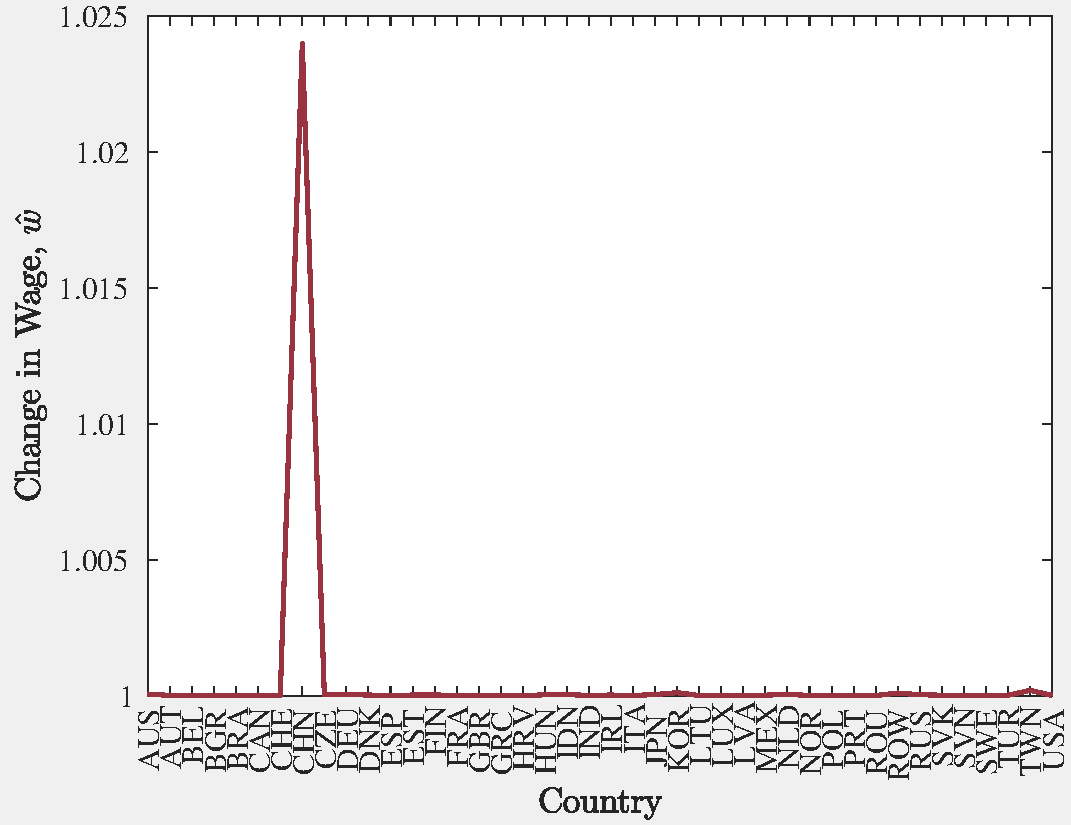
\includegraphics[width=\textwidth]{Figures/w_hat.pdf}
            \caption{US numeraire}
        \end{subfigure}
        \begin{subfigure}[b]{0.47\textwidth}
            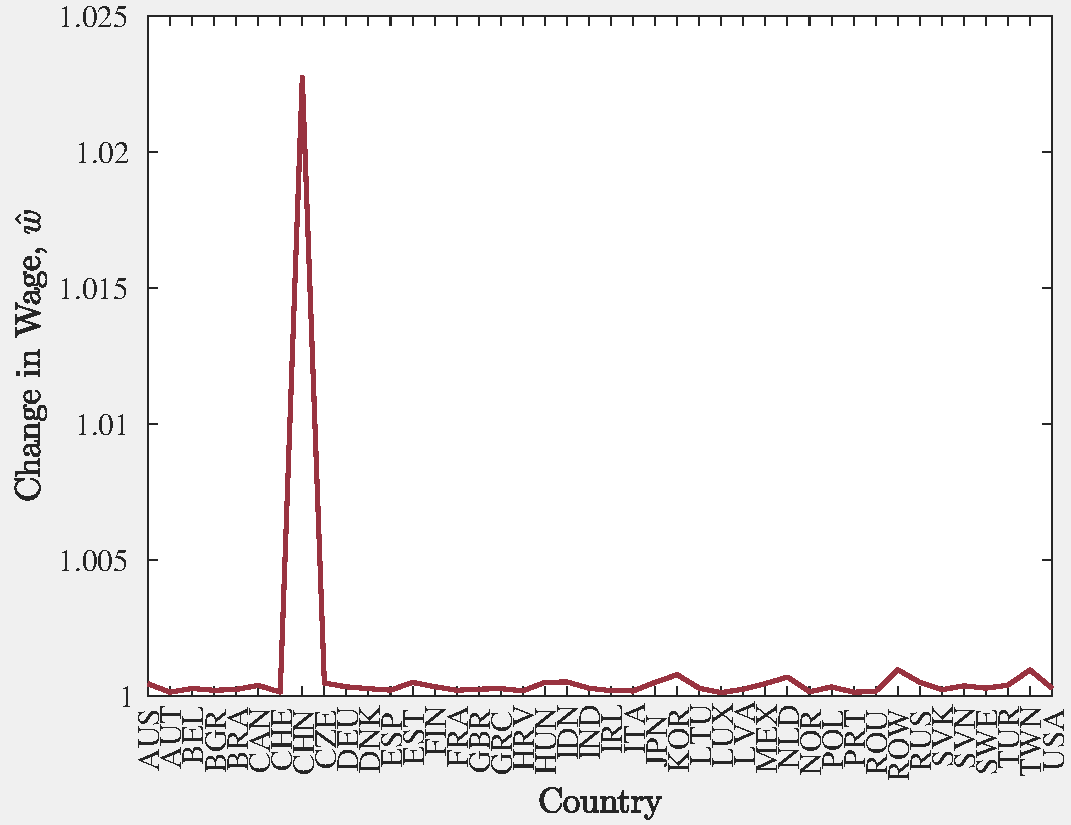
\includegraphics[width=\textwidth]{Figures/w_hat2.pdf}
            \caption{China Numeraire}
        \end{subfigure}
\end{figure}
\end{enumerate}
\clearpage

\section{EK extension with multiple sectors and trade in intermediate goods}

We now consider a version of the model in Caliendo and Parro (2015). Our goal is to evaluate how the impact of trade and productivity shocks differs when we allow for trade in intermediate goods.
\begin{enumerate}[label=\roman*., leftmargin=*]
    \item The first step is to derive the exact hat-algebra version of the non-linear system of equations that determines changes in wages as a function of initial and final levels of import tariffs, $\left(\tau_{n i}^{j, 0}\right.$ and $\left.\tau_{n i}^{j, 1}\right)$, trade cost shocks $\left(\hat{d}_{n i}\right)$, productivity shocks $\left(\hat{T}_{n}\right)$, transfer shocks $\left(\hat{D}_{n}\right)$, parameters $\left\{\gamma_{n}^{j k}, \alpha_{n}^{j}, \theta^{j}\right\}$, and the initial matrix of sector-level trade flows $\left(X_{n i}^{j, 0}\right)$. Specifically, starting from the equilibrium system in the lecture slides show that

\begin{enumerate}
    \item The change in the price index solves

\begin{equation*}
\hat{P}_{n}^{j}=\left(\sum_{i} \pi_{n i}^{j, 0}\left(\hat{\tau}_{n i}^{j}\left(\hat{w}_{i}\right)^{\gamma_{i}^{j}} \Pi_{k}\left(\hat{P}_{i}^{k}\right)^{\gamma_{i}^{kj}}\right)^{-\theta^{j}}\right)^{-1 / \theta^{j}},
\end{equation*}
where $\hat{\tilde{\tau}}_{n i}^{j}=\left(1+\tau_{n i}^{j, 1}\right) /\left(1+\tau_{n i}^{j, 0}\right)$.
\item[Sol.] Begin with the equilibrium price formula 
\begin{equation*}
    P_n^j = A^j \left( \sum_i \lambda_i^j \left((1+\tau_{ni}) d_{ni}^j\right)^{-\theta^j} \left((w_i)^{\gamma_i^j} \prod_k (P_i^k)^{\gamma_i^{kj}}\right)^{-\theta^j} \right)^{-\frac{1}{\theta^j}} 
\end{equation*}
As before, begin by multiplying and dividing by the equilibrium the price index
\begin{align*}
    \hat{P}_n^j &= \frac{A^j}{{P_n^j}^0 }\left( \sum_{i=1}^N {\lambda_i^j}^0 \hat{\lambda}_i^j \left(\hat{\tau}_{ni} {\tau_{ni}}^0 {d_{ni}^j}^0 \hat{d}_{ni}^j\right)^{-\theta^j} \left((\hat{w}_i {w_i}^0)^{\gamma_i^j} \prod_k (\hat{P}_i^k {P_i^k}^0)^{\gamma_i^{kj}}\right)^{-\theta^j} \right)^{-\frac{1}{\theta^j}} \\
    &= \frac{A^j}{A^j\left({{\Phi_n^j}^0}\right)^{-\frac{1}{\theta^j}}} \left( {\Phi^j_n}^0 {\pi_{ni}^j}^0 \sum_i \hat{\lambda}_i^j \left(\hat{\tau}_{ni} \hat{d}_{ni}^j\right)^{-\theta^j} \left((\hat{w}_i )^{\gamma_i^j} \prod_k (\hat{P}_i^k )^{\gamma_i^{kj}}\right)^{-\theta^j} \right)^{-\frac{1}{\theta^j}} \\
    &= \left( {\pi_{ni}^j}^0 \sum_i \hat{\lambda}_i^j \left(\hat{\tau}_{ni} \hat{d}_{ni}^j\right)^{-\theta^j} \left((\hat{w}_i )^{\gamma_i^j} \prod_k (\hat{P}_i^k )^{\gamma_i^{kj}}\right)^{-\theta^j} \right)^{-\frac{1}{\theta^j}} 
\end{align*}

\item  The change in the share of spending in sector $j$ of country $n$ on goods from country $i$ is given by

\begin{equation*}
\hat{\pi}_{n i}^{j}=\left(\hat{\tau}_{n i}^{j}\left(\hat{w}_{i}\right)^{\gamma_{i}^{j}} \Pi_{k}\left(\hat{P}_{i}^{k}\right)^{\gamma_{i}^{k j}}\right)^{-\theta^{j}}\left(\hat{P}_{n}^{j}\right)^{\theta^{j}} .
\end{equation*}

\item[Sol.] I am gonna jump straight ahead into the algebra because this pset is insane a long 
\begin{align*}
    \hat{\pi}_{ni}^j &= \frac{\hat{\lambda}_i^j {\lambda_i^j}^0 \left({\tau_{ni}}^0d_{ni}^{j0}\hat{\tau}_{ni}\hat{d}_{ni}^j\right)^{-\theta^j} \left((w_i^0 \hat{w}_i)^{\gamma_i^j} \prod_k (P_i^{k0} \hat{P}_i^k)^{\gamma_i^{k,j}}\right)^{-\theta^j}}{\pi_{ni}^{j0}({P_n^j}^0 \hat{P}_n^j/A^j)^{-\theta^j}} \\
    &= \frac{\hat{\lambda}_i^j  \left(\hat{\tau}_{ni}\hat{d}_{ni}^j\right)^{-\theta^j} \left((\hat{w}_i)^{\gamma_i^j} \prod_k ( \hat{P}_i^k)^{\gamma_i^{k,j}}\right)^{-\theta^j}}{({ \hat{P}_n^j)^{-\theta^j}}}
\end{align*}

\item The change in spending in sector $j$ of country $n$ on goods from country $i$ is given by the solution of
\begin{equation*}
X_{n i}^{j, 0} \hat{X}_{n i}^{j}=\hat{F}_{n i}^{j}+\pi_{n i}^{j, 0} \hat{\pi}_{n i}^{j} \sum_{k} \sum_{d}\left(\frac{\alpha_{n}^{j} \tau_{n d}^{k, 1}}{1+\tau_{n d}^{k, 1}} X_{n d}^{k, 0} \hat{X}_{n d}^{k}+\frac{\gamma_{n}^{j k}}{1+\tau_{d n}^{k, 1}} X_{d n}^{k, 0} \hat{X}_{d n}^{k}\right),
\end{equation*}
where
\begin{equation*}
\hat{F}_{n i}^{j} \equiv \pi_{n i}^{j, 0} \hat{\pi}_{n i}^{j} \alpha_{n}^{j}\left(\left(w_{n}^{0} L_{n}^{0}\right) \hat{w}_{n} \hat{L}_{n}+\left(h\left(w^{0}\right) D_{n}^{0}\right) \frac{h\left(w^{0} \hat{w}\right)}{h\left(w^{0}\right)} \hat{D}_{n}\right)
\end{equation*}
with $h(w)$ the numeraire of international transfers. Henceforth, we set the numeraire of transfers to be the US wage: $h(w)=w_{\text {US }}$ and $\frac{h\left(w^{0} \hat{w}\right)}{h\left(w^{0}\right)}=\hat{w}_{\text {US. }}$.

\item The labor market clearing condition is

\begin{equation*}
\hat{w}_{i} \hat{L}_{i}=\sum_{n} \sum_{j} \frac{\gamma_{i}^{j}}{1+\tau_{n i}^{j, 1}} \frac{X_{n i}^{j, 0} \hat{X}_{n i}^{j}}{w_{i}^{0} L_{i}^{0}} .
\end{equation*}
\item[Sol.] Labor market clearing is
\begin{equation*}
    w_n L_n = \sum_j \gamma_n^j \sum_d \frac{1}{1+\tau_{ni}^k} X_{ni}^k 
\end{equation*}
This is a one-trick pony. Multiply and divide to get 
\begin{equation*}
    \hat{w}_i \hat{L}_i = \sum_n \sum_j \frac{\gamma_i^j}{1+{\tau_{ni}^j}^1} \frac{{X_{ni}^j}^0 \hat{X}_{ni}^j}{{w_i}^0{L_i}^0}
\end{equation*}

\end{enumerate}

\item Download the file "bilateral\_trade\_sector\_country.csv" from the same link. It was again built from the 2014 WIOT Table. The variable trade\_flow2014 is the value of trade flows, $\tilde{X}_{n i}^{j k}$, from an origin sector $j$ and country $i$ (sector\_org and country\_org) to another destination sector $k$ country $n$ (sector\_dest and country\_dest). You can find the list of sectors in "sector\_list.csv".
\begin{enumerate}
    \item We calibrate the initial equilibrium tariffs to be zero: $\tau_{n i}^{j, 0}=0$ for all $j$ and $n i$.

\item Compute $X_{n i}^{j, 0}$ as the sum of the trade flows in 2014 for each country pair $n i$ and sector $j: X_{n i}^{j, 0}=\sum_{k} \tilde{X}_{n i}^{j k}$. Use trade flows to compute spending shares, $\pi_{n i}^{j, 0}=$ $X_{n i}^{j, 0} / \sum_{o} X_{n o}^{j, 0}$

\item Compute $\gamma_{n}^{j k}$ as the ratio between the purchases of sector $k$ in country $n$ on goods of sector $j$ (from all origin countries) and the total revenue of sector $k$ in country $n: \gamma_{n}^{j k}=\sum_{i} \tilde{X}_{n i}^{j k} / \sum_{i} X_{i n}^{k, 0}$. If the output of sector $k$ in country $n$ is zero, impute $\gamma_{n}^{j k}$ for that sector-country as the average $\gamma_{i}^{j k}$ across other countries $i$. Note that this imputation is not important, since it will not affect results. Report a heat map of the average spending shares across sectors, $\bar{\gamma}^{j k} \equiv \frac{1}{N} \sum_{n=1}^{N} \gamma_{n}^{j k}$. What sectors seem to be more important sources of inputs?
\begin{figure}[htb]
    \centering
    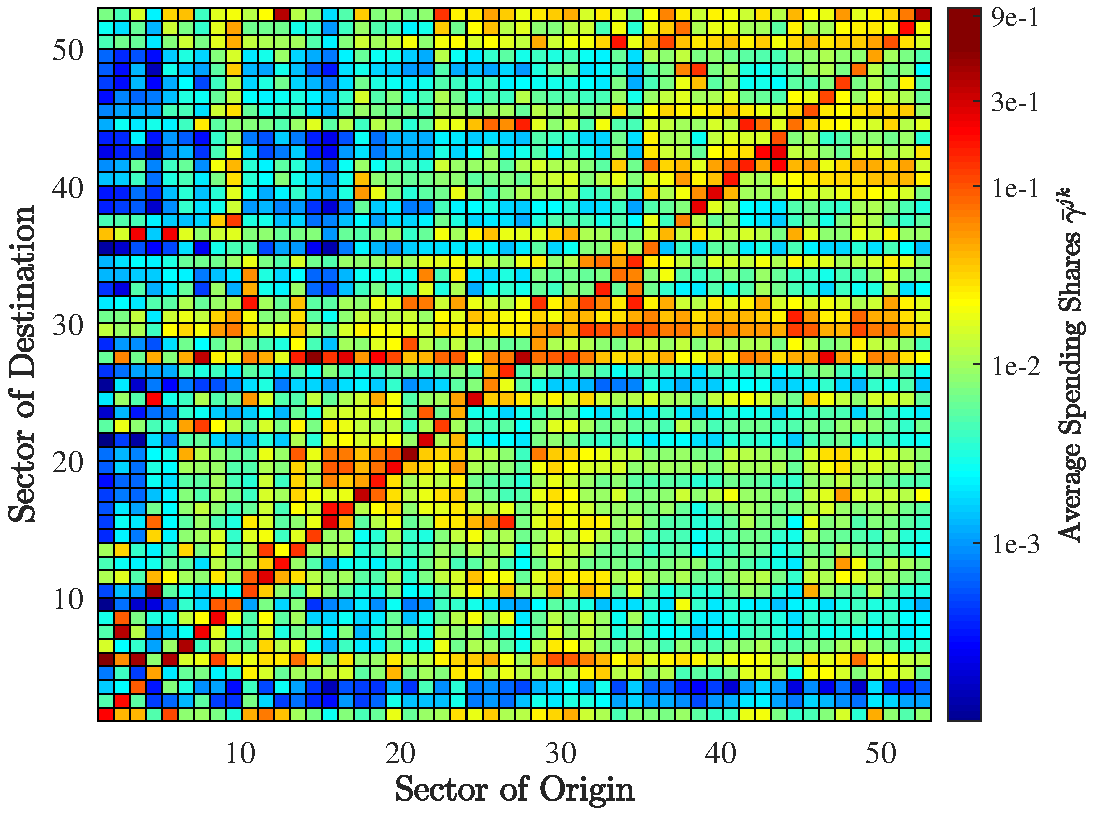
\includegraphics[width=0.7\textwidth]{Assignment 2/Figures/heatmap-ic.pdf}
    \caption{Heat Map}
\end{figure}
\FloatBarrier
\item Define $\gamma_{n}^{k} \equiv 1-\sum_{j=1}^{J} \gamma_{n}^{j k}$. Report a histogram of the share of value-added in production. What are the sectors with the highest and lowest average valueadded shares across countries?
\item[Sol.] \begin{figure}[htb]
    \centering
    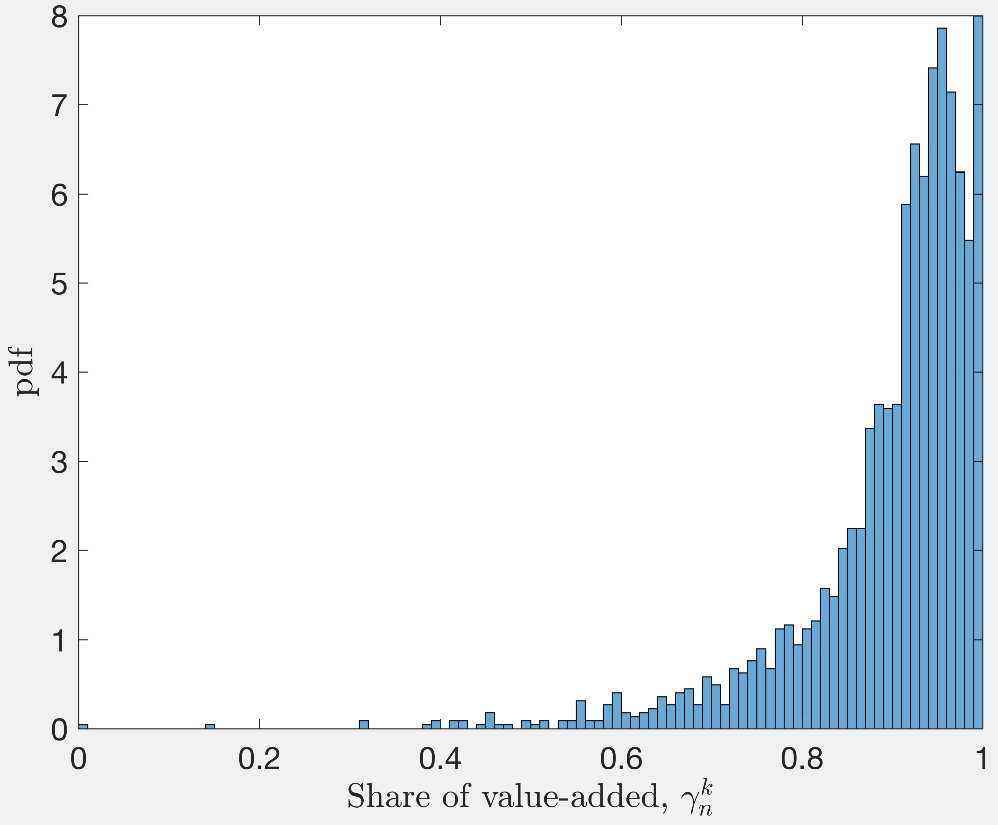
\includegraphics[width=0.45\textwidth]{Assignment 2/Figures/pdf-id.pdf}
    \caption{PDF}
\end{figure}
\FloatBarrier
\item Use the factor market clearing condition to compute value-added in the initial equilibrium:

\begin{equation*}
w_{i}^{0} L_{i}^{0}=\sum_{n} \sum_{j} \frac{\gamma_{i}^{j}}{1+\tau_{n i}^{j, 0}} X_{n i}^{j, 0}
\end{equation*}

Note that this procedure guarantees that the factor market clearing condition holds in the initial equilibrium.
\item[Sol.] \textcolor{blue}{See code}

\item Use the good market clearing condition in the initial equilibrium to show that you can compute international transfers as

\begin{equation*}
h\left(w^{0}\right) D_{n}^{0}=\sum_{k} \sum_{d} \frac{X_{n d}^{k, 0}}{1+\tau_{n d}^{k, 0}}-\sum_{k} \sum_{d} \frac{X_{d n}^{k, 0}}{1+\tau_{d n}^{k, 0}} .
\end{equation*}

Report a histogram of international transfers as a share of value-added, $h\left(w^{0}\right) D_{n}^{0} / w_{n}^{0} L_{n}^{0}$.

What are the countries with the highest and lowest transfer-to-income ratio?
\item[Sol.] \textcolor{blue}{See code}

\item Finally, use again the good market clearing condition to show that you can calibrate final spending shares as

\begin{equation*}
\alpha_{n}^{j}=\frac{\sum_{i} X_{n i}^{j}-\sum_{k} \sum_{d}\left(\frac{\gamma_{n}^{j k}}{1+\tau_{d n}^{k, 0}} X_{d n}^{k, 0}\right)}{w_{n}^{0} L_{n}^{0}+R_{n}^{0}+h\left(w^{0}\right) D_{n}^{0}}
\end{equation*}

where $R_{n}^{0}=\sum_{i} \sum_{k} \frac{\tau_{n i}^{k, 0}}{1+\tau_{n i}^{k, 0}} X_{n i}^{k, 0}$ is the initial tariff revenue. Note that this procedure guarantees that the good market clearing condition holds in the initial equilibrium. Compute the average spending shares across sectors, $\bar{\alpha}^{j}=$ $\frac{1}{N} \sum_{n=1}^{N} \alpha_{n}^{j}$. What sectors seem to be more important for final consumption?
\item[Sol.] \textcolor{blue}{See code}

\item Calibrate $\theta^{j}$ using the values in Caliendo and Parro (2015). If a sector is not in their list, set the parameter to the average across sectors reported in the last row of their main table of estimates.
\end{enumerate}

iii. Implement the following algorithm to compute counterfactual exercises.

(a) Consider steps, $b=1, \ldots, B$. Guess that $\hat{w}_{i}(b=0)=1$ for all countries.

(b) Given $\hat{w}(b)=\left\{w_{i}(b)\right\}_{i}$, compute the excess labor demand as follows.

i. We first recover the price index in each country and sector. Consider steps $v=1, \ldots, V$. Set $\hat{P}_{n}^{j}(v=0 ; b)=1$ for all $n$ and $j$.

ii. Given $\hat{P}_{n}^{j}(v ; b)$ for all $n$ and $j$, compute

\begin{equation*}
\hat{\hat{P}}_{n}^{j}(v ; b)=\left(\sum_{i} \pi_{n i}^{j, 0}\left(\hat{\tau}_{n i}\left(\hat{w}_{i}(b)\right)^{\gamma_{i}^{j}} \Pi_{k}\left(\hat{P}_{i}^{k}(v ; b)\right)^{\gamma_{i}^{k j}}\right)^{-\theta^{j}}\right)^{-1 / \theta^{j}}
\end{equation*}

If $\max _{n, j}\left\{\left|\hat{\hat{P}}_{n}^{j}(v ; b)-\hat{P}_{n}^{j}(v ; b)\right|\right\}<$ tol, then stop. Otherwise, compute a new guess with

\begin{equation*}
\hat{P}_{n}^{j}(v+1 ; b)=\hat{P}_{n}^{j}(v ; b)+\kappa^{p}\left(\hat{\hat{P}}_{n}^{j}(v ; b)-\hat{P}_{n}^{j}(v ; b)\right)
\end{equation*}

where $\kappa^{p}$ is a positive constant. You can start with $\kappa^{p}=1$, and reduce it if the algorithm does not converge for a given $\hat{w}(b)$. Let $\hat{P}(b) \equiv\left\{\hat{P}_{n}^{j}(v ; b)\right\}_{n=1, j=1}^{N, I}$ denote the change in price indices for which the algorithm converges.

iii. Given $\hat{w}(b)$ and $\hat{P}(b)$, compute $\hat{\pi}_{n i}^{j}(b)$ using (5). Then use it to compute changes in bilateral trade flows in each sector, $X_{n i}^{j, 0} \hat{X}_{n i}^{j}$, as the solution of the linear system in (6). Specifically, note that you can compute $\hat{F}_{n i}^{j}(b)$ from (7), and then solve for $X^{0} \hat{X}(b) \equiv\left\{X_{n i}^{j, 0} \hat{X}_{n i}^{j}(b)\right\}_{n=1, i=1, j=1}^{N, N, J}$ using the linear system

\begin{equation*}
\sum_{d, o, k} \beta_{n i j, d o k}\left(X_{d o}^{k, 0} \hat{X}_{d o}^{k}(b)\right)=\hat{F}_{n i}^{j}(b), \quad \forall n, i, j
\end{equation*}

where

\begin{equation*}
\beta_{n i j, d o k} \equiv 1[n i j=d o k]-\pi_{n i}^{j, 0} \hat{\pi}_{n i}^{j}(b)\left(\frac{\alpha_{n}^{j} \tau_{d o}^{k, 1}}{1+\tau_{d o}^{k, 1}} 1[d=n]+\frac{\gamma_{n}^{j k}}{1+\tau_{d o}^{k, 1}} 1[o=n]\right)
\end{equation*}

with $1[n i j=$ dok $], 1[d=n]$ and $1[0=n]$ denoting dummy variables. Note that, since $\sum_{n i j} \beta_{n i j, d o k}=\frac{\gamma_{o}^{k}}{1+\tau_{d}^{k, 1}} \in(0,1)$, the square matrix $\beta \equiv\left[\beta_{n i j, d o k}\right]_{n i j, d o k}$ with dimension $N N J \times N N J$ is invertible. Optional: show that $\sum_{n i j} \beta_{n i j, d o k}=$ $\frac{\gamma_{o}^{k}}{1+\tau_{o d}^{k, 1}}$, and then use this statement to establish the invertibility of $\beta$ and to check your code.

iv. Given $\hat{w}(b)$ and $X^{0} \hat{X}(b)$, compute the excess labor demand implied by the labor market clearing in (8):

\begin{equation*}
Z_{i}(\hat{w}(b))=\sum_{n} \sum_{j} \frac{\gamma_{i}^{j}}{1+\tau_{n i}^{j, 1}} \frac{X_{n i}^{j, 0} \hat{X}_{n i}^{j}(b)}{w_{i}^{0} L_{i}^{0}}-\hat{w}_{i}(b) \hat{L}_{i} .
\end{equation*}

(c) If $\max _{i \neq \mathrm{US}}\left\{\left|Z_{i}(\hat{w}(b))\right|\right\}<t o l$, then stop. Otherwise, compute a new guess for $i \neq \mathrm{US}$ :

\begin{equation*}
\hat{w}_{i}(b+1)=\hat{w}_{i}(b)+\kappa^{w} Z_{i}(\hat{w}(b))
\end{equation*}

where $\kappa^{w}$ is a positive constant.

(d) Compute changes in the real wage $\left(\hat{w}_{n} / \hat{P}_{n}\right)$ and real expenditure $\left(\hat{X}_{n} / \hat{P}_{n}\right)$.

\item Assume that the US wage is the numeraire (i.e., $w_{\mathrm{US}}^{0}=\hat{w}_{\mathrm{US}}=1$ ). Compute the impact of a $10 \%$ increase in Chinese productivity in all sectors, $\hat{T}_{\text {China }}^{j}=1.1$ for all $j$, on the wage (relative to the US wage), real wage, and real expenditure of each country. Compare your results to those obtained in item 1.iii above, and provide a brief intuition for the differences.

\item Assume that the US wage is the numeraire (i.e., $w_{\mathrm{US}}^{0}=\hat{w}_{\mathrm{US}}=1$ ).

(a) Compute the impact of a 10\% increase in US import cost from all countries and sectors, $\hat{d}_{\mathrm{US} i}^{j}=1.1$ for all $i$ and $j$, on the wage (relative to the US wage), real wage, and real expenditure of each country.

(b) Compute the impact of a 10\% increase in US import tariffs from all countries and sectors, $\hat{\tau}_{\mathrm{US} i}^{j}=1.1$ for all $i$ and $j$, on the wage (relative to the US wage), real wage, and real expenditure of each country. Note that, since $\hat{\hat{\tau}}_{\mathrm{US} i}^{j}=(1+$ $\left.\tau_{\mathrm{US} i}^{j, 1}\right) /\left(1+\tau_{\mathrm{US} i}^{j, 0}\right)$ and $\tau_{\mathrm{US} i}^{j, 0}=0$ (in our calibration defined in 2.ii.a), the shock is equivalent to setting the new US tariffs to $10 \%, \tau_{\mathrm{US} i}^{j, 1}=0.1$.

(c) Compare the impact of both policies on the US and other countries. Provide a brief intuition for the differences.

\end{enumerate}

\end{document}
